\begin{frame}
    \frametitle{Exemples}
    
    \begin{columns}[T] % L'option [T] aligne le contenu en haut des colonnes
        
        \begin{column}{0.5\textwidth}
            \begin{figure}
                
\includegraphics[width=\linewidth]{6-Resultats/classic/perturbation/distance.pdf}
                \caption{Interdistance entre robots au cours du temps.}
                \label{fig:gauche}
            \end{figure}
        \end{column}
        
        \begin{column}{0.5\textwidth}
            \begin{figure}
                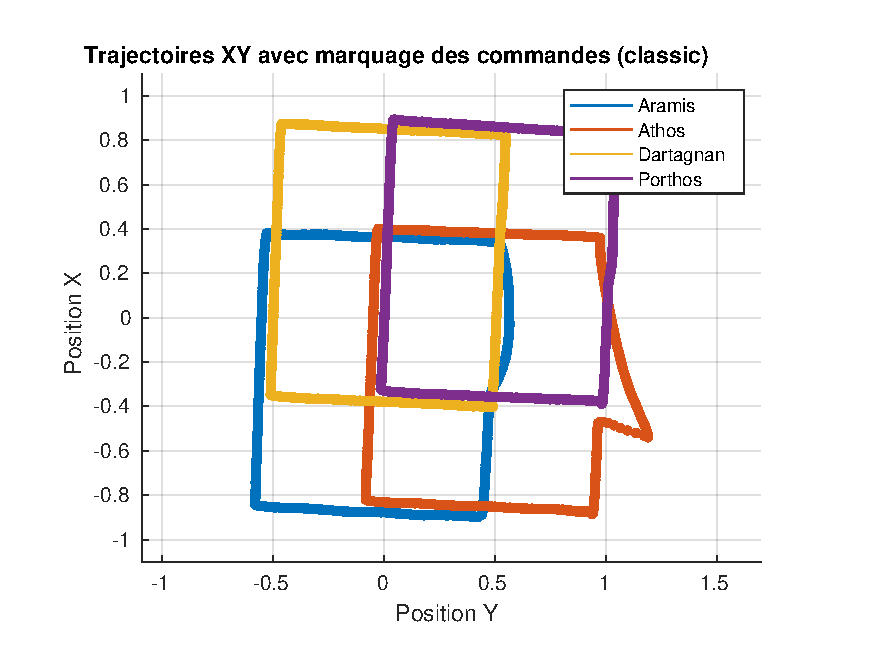
\includegraphics[width=\linewidth]{6-Resultats/classic/perturbation/trajectoires_marquage.pdf}
                \caption{Trajectoires}
                \label{fig:droite}
            \end{figure}
        \end{column}
        
    \end{columns}
    
\end{frame}

\begin{frame}
    \frametitle{Exemples}
    
    \begin{columns}[T] % L'option [T] aligne le contenu en haut des colonnes
        
        \begin{column}{0.5\textwidth}
            \begin{figure}
                
\includegraphics[width=\linewidth]{6-Resultats/ev/perturbation/distance.pdf}
                \caption{Interdistance entre robots au cours du temps.}
                \label{fig:evgauche}
            \end{figure}
        \end{column}
        
        \begin{column}{0.5\textwidth}
            \begin{figure}
                
\includegraphics[width=\linewidth]{6-Resultats/ev/perturbation/trajectoires_marquage.pdf}
                \caption{Trajectoires}
                \label{fig:evdroite}
            \end{figure}
        \end{column}
        
    \end{columns}
    
\end{frame}